%%%%%%%%%%%%%%%%%%%%%%%%%%%%%%%%%%%%%%%%%%%%%%%%%%%%%%%%%%%%
%
% Section: Functions and Graphs
%
%%%%%%%%%%%%%%%%%%%%%%%%%%%%%%%%%%%%%%%%%%%%%%%%%%%%%%%%%%%%
\section{Functions and Graphs}
\label{FunctionsandGraphs}

As we saw in the preceding section, functions can be represented in many different ways. If a rule gives one and only one output for each input, it’s a function, whether we specify that rule using a formula, a description, a table, or some other means.\\

In this section we’ll discuss another tool for describing, and working with, functions. You probably already have some experience work working with this tool, but in this section we’ll develop the idea of a graph in the framework of functions. If some of this section is old news to you, you’ll still want to walk through this carefully, to see how graphs and functions are related to each other. If, on the other hand, you don’t have much experience with them, don’t panic – we’ll build everything from the ground up.

%%%%%%%%%%%%%%%%%%%%%%%%%%%%%%%%%%%%%%%%%%%%%%%%%%%%%%%%%%%%
%
% Subsection: Functions and Coordinates
%
%%%%%%%%%%%%%%%%%%%%%%%%%%%%%%%%%%%%%%%%%%%%%%%%%%%%%%%%%%%%

\subsection{Functions and Coordinates}

We’ve already discussed the use of tables as a way of describing a function. A table is simply an organized list of the inputs for a function together with their outputs. An alternative way of doing this is to use coordinate pairs. A coordinate pair is a way of writing a given input together with its output, written in the form:

\begin{center}
	$(\text{input value}, \text{output value})$
\end{center}

For example, suppose we define a function using the following table:

\begin{center}
	\begin{tabular}{c|c|c|c|c}
		$x$ & $0$ & $1$ & $2$ & $3$\\
		\hline
		$f(x)$ & $5$ & $4$ & $9$ & $-2$ 
	\end{tabular}
\end{center}

We could also define this function with a list of coordinate pairs for each input and output. The table tells us that for the input $x=0$ we get the output $f(0)=5$. As a coordinate pair, we would write this as $(0,5)$. Likewise, we could express the fact that $f(1)=4$ by writing the coordinate pair $(1,4)$. And so on. Listing out the remaining inputs and outputs in the same way, we could represent this function as a set of coordinate pairs:

$$\{(0,5),(1,4),(2,9),(3,-2)\}$$

(the curly brackets are used to indicate that this is a set of coordinate pairs).

\exam{\label{FunctionsandGraphsExample1}Rewrite the function given in the table below as a set of coordinate pairs.
	\begin{center}
		\begin{tabular}{c|c|c|c|c|c}
			$x$ & 4 & 7 & 3 & 9 & 1 \\
			\hline
			$g(x)$ & 0 & 0 & 2 & -4 & 6
		\end{tabular}
	\end{center}
}

\indenttext{
	Following the pattern of $(\text{input}, \text{output})$ we would write $\{(4,0), (7,0), (3,2), (9, -4), (1,6)\}$.
}

\exam{\label{FunctionsandGraphsExample2}
	Suppose that for a given function $h(3)=5$.  Express this as a coordinate pair.
}

\indenttext{
	Following the pattern again, we would write this as the coordinate pair $(3,5)$.
}

\bigskip

You may notice that coordinate pairs look an exactly like interval notation, $(3,5)$ read as a coordinate pair means \quotes{the input $3$ gives the output $5$}; but $(3,5)$ read as an interval means \quotes{all the real numbers between $3$ and $5$ not including $3$ and $5$ themselves.} It is really unfortunate that the same notation can be correctly interpreted as two completely different things. Fortunately, though, this is almost never a problem because it is just about always clear from context whether we are talking about a coordinate pair or an interval.\\

Any function that can be described with a table can be described with coordinate pairs. And so, anything we can do with a function as a table we can do with a function as a set of coordinate pairs.

\exam{\label{FunctionsandGraphsExample3}
	Is $\{(0,3), (1,3), (2,5), (3,6), (5,11)\}$ a function?
}

\indenttext{
	In this set of coordinate pairs, each distinct input has one and only one output. Therefore this is a
	function.
}

\exam{\label{FunctionsandGraphsExample4}
	Is $\{(0,5), (1,-3), (3,6), (-2,7), (1,0)\}$ a function?
}

\indenttext{
	In this set of coordinate pairs we have both $(1,-3)$ and $(1,0)$. This means that the input $1$ gets both $-3$ and $0$ as outputs. A function cannot give two different outputs for the same input. This is not a function.
}

%%%%%%%%%%%%%%%%%%%%%%%%%%%%%%%%%%%%%%%%%%%%%%%%%%%%%%%%%%%%
%
% Subsection: Graphs
%
%%%%%%%%%%%%%%%%%%%%%%%%%%%%%%%%%%%%%%%%%%%%%%%%%%%%%%%%%%%%

\subsection{Graphs}

Tables, and lists of coordinate pairs, both are very limited. If we are working with a function that has just a few possible inputs, then tables and lists of coordinate pairs are a simple and efficient way of giving the function. But if a function has a big domain with lots of possible inputs, producing a table or a list of coordinate pairs is impractical if not impossible.\\

For example, let’s start by considering a fairly simple function, the doubling function $f(x)=2x$.  The domain of this function is all real numbers – if we give this function any real number at all, the function can double it and give us the result as an output.\\

We could give some \underline{sample} values of this function in a table, such as this:

\begin{center}
	\begin{tabular}{c|c|c|c|c|c|c}
		x & 0 & 1 & 2 & 3 & 4 & 5 \\
		\hline
		f(x) & 0 & 2 & 4 & 6 & 8 & 10	
	\end{tabular}
\end{center}

which might be useful to give a sense, by examples, of just what this function does. But this table does not fully describe the function, because it only gives the outputs for the comparatively few selected inputs listed in the table. We might assume from this table what the outputs would be for other inputs, but we could not, just from this table, know for sure. This table certainly looks like we’ve got the doubling function in mind. It certainly looks like if we input $6$ we’d get an output of $12$. But we can’t tell for sure. This table only tells us the outputs for the specific inputs listed.\\

On the face of it, it seems like it would be impossible to create a table that would list all infinitely many inputs and outputs for the doubling function. But, it turns out that there actually is a way to do this. How do you make a list of all the real numbers? Well, in fact you already know a way of doing this: by drawing a number line.\\

A number line \quotes{lists} all the real numbers because every real number corresponds to a point on the line. Some of the numbers, such as $-3$, $0$ and $5$ are marked specifically on the number line below.  But we understand the other numbers are there as well. Where is $4.75$?\\

Well, we understand it to be at the point $\frac{3}{4}$ of the way between 4 and 5. Where is $-3,000,000$?\\

Well, we understand that arrow to the left to mean the line continues forever, and so it eventually gets to the right place.

\begin{figure}[H]
	\centering
	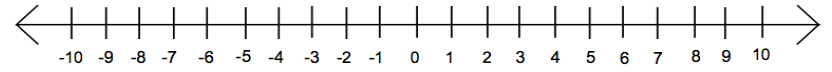
\includegraphics[width=\textwidth]{Sections/FunctionsandGraphsImages/Figure01.png}
	\caption{A visualization of all real numbers}
\end{figure}

\begin{figure}[H]
	\centering
	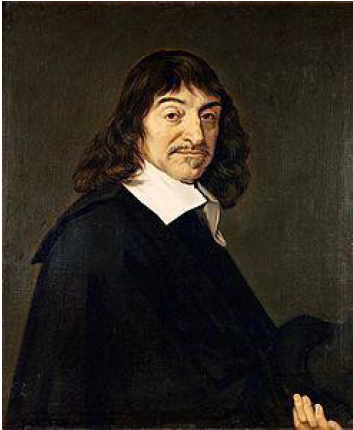
\includegraphics[scale=1.0]{Sections/FunctionsandGraphsImages/Figure02.png}
	\caption{Descartes: He thought, therefore he was. Source: wikipedia.org}
\end{figure}

Descartes’ innovation was to draw two number lines, one perpendicular to the other, to create a plane, called the \textbf{coordinate plane}\index{Coordinate Plane}, or, in his honor, the \textbf{Cartesian plane}\index{Cartesian Plane} \footnote{\quotes{Cartesian} is derived from the name \quotes{Descartes}. The \quotes{Des} is left off for reasons having to do with the Latin form of his name.}. The horizontal number line is used to represent all the possible input values of a function. It is known as the \textbf{horizontal axis, or the input axis}\index{Coordinate Plane!Horizontal Axis}, or, since the most common variable name to use for inputs is $x$, the \textbf{$x$-axis}.\\

The output values for the function are represented using the vertical number line, known as the \textbf{vertical axis, or output axis}\index{Coordinate Plane!Vertical Axis}, or, since the most common variable name to use for outputs is $y$, \textbf{the $y$-axis}.

\begin{figure}[H]
	\centering
	%should be scaled down
	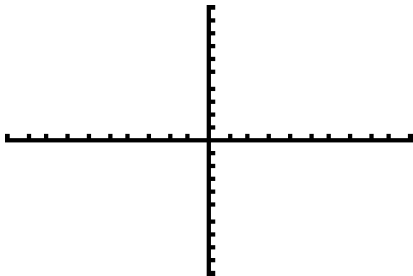
\includegraphics[scale=1.0]{Sections/FunctionsandGraphsImages/Figure03.png}
	\caption{A set of coordinate axes.}
\end{figure}

Any coordinate pair can be represented as a point in this plane. The $x$ and $y$ values of the coordinate pair give its point’s location. We move right or left along the $x$-axis to the $x$ value, and then from there we move up or down parallel to the $y$-axis to the $y$ value. For example, the coordinate pair $(3, -2)$ would be represented by the point in the plane shown below:

\begin{figure}[H]
	\centering
	%should be scaled down
	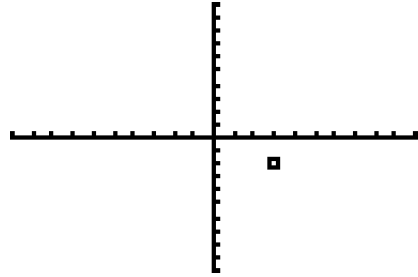
\includegraphics[scale=1.0]{Sections/FunctionsandGraphsImages/Figure04.png}
	\caption{The point $(3,-2)$ marked on a set of axes.}
\end{figure}

Now, we can represent any numerical table as a collection of points in the plane. The table we create above, giving a few selected inputs and outputs for the function $f(x)=2x$ could be represented by the following points in the plane:

\begin{figure}[H]
	\centering
	%should be scaled down
	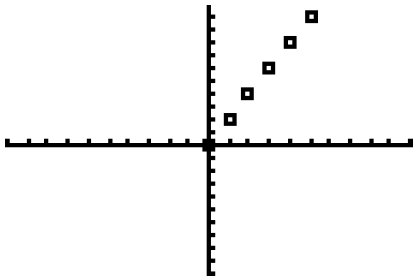
\includegraphics[scale=1.0]{Sections/FunctionsandGraphsImages/Figure05.png}
	\caption{Some input-output pairs for $f(x)=2x$.}
\end{figure}

Now here’s the infinitely clever part. If we want to represent all the input-output pairs for a function, we can actually do that. Notice that the points we plotted for $f(x)=2x$ in the diagram above all seem to fall into a pattern – they seem to fall in a straight line. It turns out that if we plotted all the input-output pairs for $f(x)=2x$ they would form a straight line like this:

\begin{figure}[H]
	\centering
	%should be scaled down
	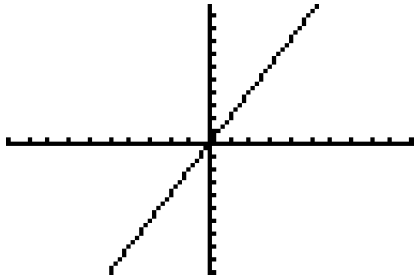
\includegraphics[scale=1.0]{Sections/FunctionsandGraphsImages/Figure06.png}
	\caption{The line formed by input-output pairs for $f(x)=2x$.}
\end{figure}

Note that for the time being, you’ll have to take it on faith that all the input-output pairs for this function actually do fall into this line; in the next chapter we’ll see how we know for sure that the input-output pairs are precisely the same as the points on the line. It should though seem
reasonable to expect there is something more than just a coincidence going on that the points we plotted happen to fit a straight line.\\

For many functions, the points for all the input-output pairs will form straight lines like this one. There are other possibilities, however. For example, if we consider the function $g(x)=x^2$ we can create this table:

\begin{center}
	\begin{tabular}{c|c|c|c|c|c|c|c}
		$x$ & -3 & -2 & -1 & 0 & 1 & 2 & 3\\
		\hline
		$g(x)$ & 9 & 4 & 1 & 0 & 1 & 4 & 9
	\end{tabular}
\end{center}

and if we plot the points from this table in the plane we get:

\begin{figure}[H]
	\centering
	%should be scaled down
	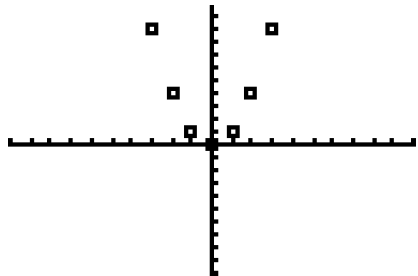
\includegraphics[scale=1.0]{Sections/FunctionsandGraphsImages/Figure07.png}
	\caption{Some of the input-output pairs for the function $g(x)=x^2$.}
\end{figure}

which clearly can’t be made to fit any straight line. It turns out (again, we’ll see exactly why this is later) that the actual collection of points for this function looks like this:

\begin{figure}[H]
	\centering
	%should be scaled down
	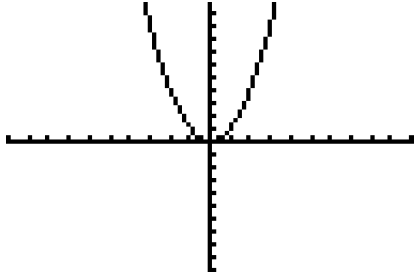
\includegraphics[scale=1.0]{Sections/FunctionsandGraphsImages/Figure08.png}
	\caption{The shape formed by the input-output pairs for $g(x)=x^2$.}
\end{figure}

Even though that’s not a straight line, it definitely fits a pattern. That’s huge. It turns out that when we plot all the points for all the input-output pairs for just about any function we might care about, the result will always be some reasonable shape or pattern.\\

The collection of all the input-output pairs for a function plotted in a coordinate plane is called a \textbf{graph}\index{Graph} of the function. We will see in the upcoming chapters of this book that graphs are an incredibly powerful tools for working with functions.\\

Before moving on, there are a few terms that are commonly used with graphs and the coordinate plane that we should define. The point $(0,0)$ that lies in the center where the two axes intersect is called the \textbf{origin}\index{Coordinate Plane!Origin}. You can think of the origin as the \quotes{starting point} from which we move to the
coordinates of other points.\\

Also, the two axes naturally divide the coordinate plan into four quarters, which are called \textbf{quadrants}\index{Coordinate Plane!Quadrants}. The quadrants are numbered, usually with Roman numerals, starting in the upper right and moving around counter-clockwise, as shown below:

\begin{figure}[H]
	\centering
	%should be scaled down
	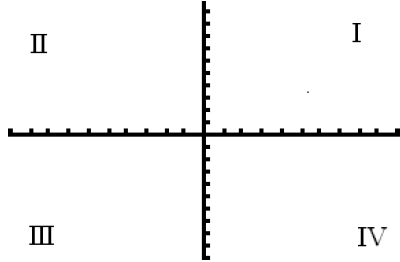
\includegraphics[scale=1.0]{Sections/FunctionsandGraphsImages/Figure09.png}
	\caption{The quadrants of the Cartesian Plane.}
\end{figure}

Quadrant I is called the \textbf{first quadrant}, quadrant II is called the \textbf{second quadrant}, etc.\\

\exam{\label{FunctionsandGraphsExample5}Sketch the location of the point $(-3,1)$ in the Cartesian plane. In which quadrant is this point located?}

\indenttext{To locate this point we follow the input (horizontal) axis from the origin to the left to $-3$ and then follow the output (vertical) axis up to a height of $+1$.

	\begin{figure}[H]
		\centering
		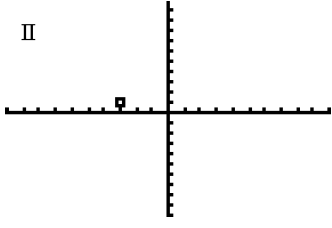
\includegraphics[scale=1.0]{Sections/FunctionsandGraphsImages/Figure10.png}
		\caption{The location of $(-3,1)$ in the Cartesian Plane}
	\end{figure}

	This point lies in the second quadrant (i.e. Quadrant II).
}

\exam{\label{FunctionsandGraphsExample6}Sketch the location of the point $(0,-2)$ in the Cartesian plane. In which quadrant is this point located?}

\indenttext{Because the first coordinate is $0$, we don’t move at all to the right or left from the origin. We then follow the output (vertical) axis down to $-2$.
	\begin{figure}[H]
		\centering
		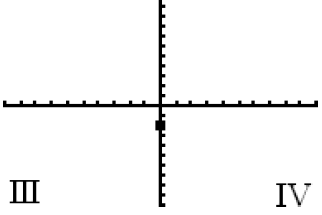
\includegraphics[scale=1.0]{Sections/FunctionsandGraphsImages/Figure11.png}
		\caption{The location of $(0,-2)$ in the Cartesian Plane}
	\end{figure}
	This point does not lie in any quadrant. It is located directly on the output (vertical) axis between Quadrants III and IV.
}

\bigskip

We can create graphs for functions whose formulas we know (more on that later). We can also, though, use graphs even without formulas as a way of describing functions. For example, suppose you are filling a tub with water at a steady rate. The amount of water in the tub is a function of the time (since at any given time there is one and only one amount of water in the tub). Can we sketch a graph of what this function would look like?\\

If we assume the starting time (when \quotes{time is zero}) is when we first started the water flowing in, we know that the graph must include the origin, since when the time is zero (i.e. when we start) the amount of water in the tub is also zero (i.e. the tub is empty). Then as time passes, the amount of water goes up at a steady rate, so our graph should also go up at a steady rate until the tub is full, at which point the graph would level off. So, the graph should look something like this:

\begin{figure}[H]
	\centering
	%should be scaled down
	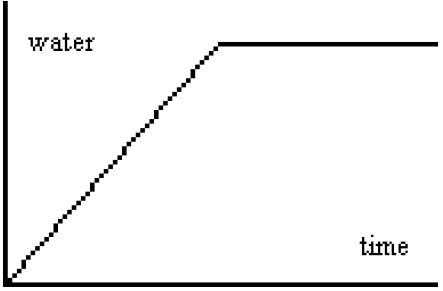
\includegraphics[scale=1.0]{Sections/FunctionsandGraphsImages/Figure12.png}
	\caption{Graph of water in the tub as a function of time}
\end{figure}

Now, we can’t put numbers on this graph because we don’t have that information; we don’t know the rate of the water’s flow, the volume of the tub, how long it took to fill, etc. But we can label the axes with the quantities each axis represents, and we can feel confident that this graph communicates the idea of filling the tub at a steady rate.\\

Notice that in this graph we only are looking at the first quadrant. This is because our interest lies only with positive values of the variables. We are not interested in the amount of water in the tub before we begin to fill it, and there could never be negative amount of water in the tub. Of course we could include show those empty quadrants if we wanted to for some reason, but doing so would serve no purpose.\\

When using a graph to describe a function you should always label the graph with as much relevant information as you have available. At a minimum, the axes should always be labeled. If other information is available, that may be included as well.

\exam{\label{FunctionsandGraphsExample7}A radioactive isotope of iodine decays with a half life of 8 hours (that is, one half of the isotope decays every 8 hours). A lab has a 20 gram sample of this isotope. Sketch a graph of the remaining amount of the isotope as a function of time.}

\indenttext{The amount is decreasing, so our graph should move downward. It cannot move down in a straight line, though, because if it did the graph would eventually fall below the horizontal axis – meaning a negative amount of iodine, which is ridiculous. So, the graph must curve downward.\\

	We can get a sense of how this would work by plotting a few points based on the information we have. Since the amount is reduced by half every 8 hours, we can figure out the amounts we have at 8 hour intervals:\\

	\begin{center}
		\begin{tabular}{c|c}
			Time (hours) & Amount (grams) \\
			\hline
			0 & 20\\
			8 & 10 \\
			16 & 5 \\
			24 & 2.5
		\end{tabular}
	\end{center}

	Roughly plotting these points:

	\begin{figure}[H]
		\centering
		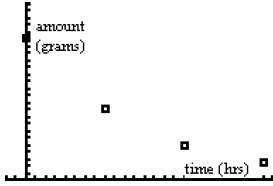
\includegraphics[scale=1.0]{Sections/FunctionsandGraphsImages/Figure13.png}
		%\caption{}
	\end{figure}

	gives us a sense of what the graph must look like. Connecting these dots into a smooth shape and labeling we should end up with a graph something like this:

	\begin{figure}[H]
		\centering
		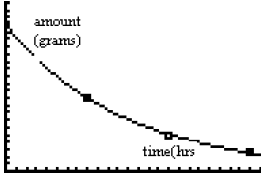
\includegraphics[scale=1.0]{Sections/FunctionsandGraphsImages/Figure14.png}
		%\caption{}
	\end{figure}

	It is not necessary and probably not even desirable to show all the plotted points specifically labeled; but it would be good to label a few values to give a sense of scale. A graph such as this would be a good choice:

	\begin{figure}[H]
		\centering
		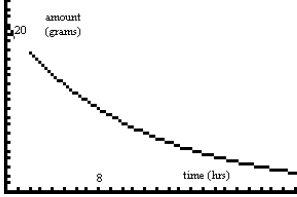
\includegraphics[scale=1.0]{Sections/FunctionsandGraphsImages/Figure15.png}
		%\caption{}
	\end{figure}
}

Graphs can take on all sorts of shapes. For example, here is graph for the closing price of the Dow Jones Industrial Average (a reflection of the US stock market) as a function of time over the years 2008-2009:

\begin{figure}[H]
	\centering
	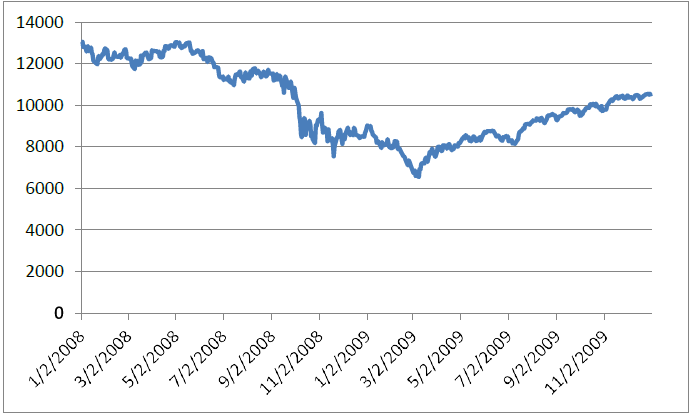
\includegraphics[scale=1.0]{Sections/FunctionsandGraphsImages/Figure16.png}
	%\caption{}
\end{figure}

And of course wilder shapes are possible. Is there any restriction on what shapes a graph can take? Well, what about a \quotes{graph} like this one:

\begin{figure}[H]
	\centering
	%should be scaled down
	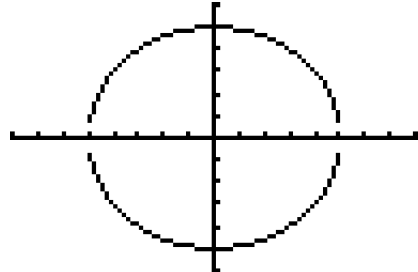
\includegraphics[scale=1.0]{Sections/FunctionsandGraphsImages/Figure17.png}
	\caption{Could this be a graph of a function?}
\end{figure}

This is a nice, smooth, geometrically pretty shape. Shapes don’t come much nicer than circles. But could it be the graph of a function? Well, no, actually. Remember that a function must give \underline{one and only one} output for each input in its domain.\\

The input $x=6$ does not have an output here, but that is fine if this were the graph of a function. That just means $6$ is not in the domain. The problem lies with inputs like $x=3$. What is the output for the input $x=3$?  Well based on where the marks on the axis are located, it looks as though the point $(3,4)$ is on the graph, so we might think the output must be $y=4$. Or, in other words, $f(3)=4$. But the point $(3,-4)$ is also appears to be on the graph, so the output for $x=3$ must also be $y=-4$. Or in other words, $f(3)=-4$ too. And that is a problem. Remember, a function must always give a straight answer! For the input $x=3$ the \quotes{graph} cannot show two different outputs. Therefore this circle cannot be the graph of a function.\\

There’s nothing special about the input $x=3$. We could have used lots of other choices for $x$ and run into the same problem. In fact, we could have used any input where the graph shows to different outputs. We don’t even need to be able to tell what the specific outputs are. If we used the input $x=-2.5$, say, we might not be able to tell very well what the corresponding outputs are, but we could tell that there are two of them.

\begin{figure}[H]
	\centering
	%should be scaled down
	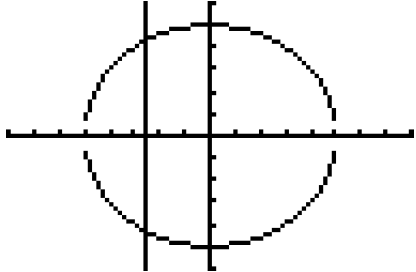
\includegraphics[scale=1.0]{Sections/FunctionsandGraphsImages/Figure18.png}
	\caption{Drawing a vertical line shows how the input value we've drawn it through has two outputs}
\end{figure}

The observation we are making here is sometimes referred to as the vertical line test.

\begin{definition}
	\index{Vertical Line Test}
	\textbf{\underline{The Vertical Line Test}}\\
	\bigskip
	A graph is the graph of a function if, and only if,\\ you can never draw a vertical line which intersects the graph more than once.\\
	\bigskip
	OR equivalently\\
	\bigskip
	A graph is the graph of a function if, and only if, \\ every vertical line you can draw will intersect the graph at most one time.
\end{definition}

Because the only requirement of a function is that it give one and only one output for each input, the only requirement for a graph to be a function is the vertical line test.

%%%%%%%%%%%%%%%%%%%%%%%%%%%%%%%%%%%%%%%%%%%%%%%%%%%%%%%%%%%%
%
% Subsection: Graphing Calculator
%
%%%%%%%%%%%%%%%%%%%%%%%%%%%%%%%%%%%%%%%%%%%%%%%%%%%%%%%%%%%%

\subsection{The Graphing Calculator}

Throughout this course, we will be using graphs extensively. A graphing calculator is required for this course, and before we conclude this section we will introduce the use of the calculator to obtain graphs of functions when we know their formulas. (We’ll just introduce the basics here, and expand on the use of the graphing calculator in future chapters.)\\

Let’s return to the function we started this chapter with, $f(x)=2x$. We can use the calculator to obtain a graph of this function using the following process.\\

\index{Calculator:Graphing}\textbf{Step 1: Enter the function formula into the calculator.} We first need to tell the calculator the formula for the function we want to graph. (We do this the same way that we entered formulas to create tables in Chapter ??.) First, hit the \quotes{Y=} key in the upper left corner of your TI-83 or 84, and then enter the formula on the first (\quotes{Y1=}) line. As with tables, the other lines (\quotes{Y2=}, \quotes{Y3=} etc.) are there to allow you to enter more than one formula at a time – not something we care about right now. Also as with tables, the formula must be written with \quotes{X} as the input variable. Use the \quotes{X,T,$\Theta$,n} key to get an \quotes{X}. The resulting screen should look like this:

\begin{figure}[H]
	\centering
	%should be scaled down
	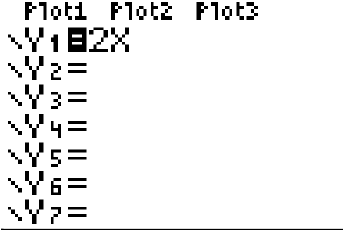
\includegraphics[scale=1.0]{Sections/FunctionsandGraphsImages/Figure19.png}
	%\caption{}
\end{figure}

\index{Calculator:Window Settings} \textbf{Step 2: Set the window.} The Cartesian plane extends out to infinity in all directions, and many graphs do as well. So of course there is no way to display the whole plane on the calculator screen.  We need to tell the calculator what portion of the plane we want it to display. \\

In the calculator’s top row there is a key labeled \quotes{WINDOW}. Hit that key now, and it will take you to a screen that should look like this (though the specific numbers you see may not be the same):

\begin{figure}[H]
	\centering
	%should be scaled down
	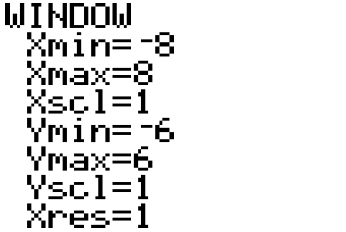
\includegraphics[scale=1.0]{Sections/FunctionsandGraphsImages/Figure20.png}
	%\caption{}
\end{figure}

The \quotes{Xmin} and \quotes{Xmax} tell the calculator the interval of $x$ (input) values to show on the graph. On the screen shown above as an example, the calculator would show the portion of the graph that lies between $x=-8$ and $x=8$. Likewise, the \quotes{Ymin} and \quotes{Ymax} determine the range of $y$ (output) values used; in this window it would be the portion of the graph that lies between $y=-6$ and $y=6$.\\

The \quotes{Xscl} and \quotes{Yscl} determine where the marks on the axes occur. These both being set to 1 tells the calculator to mark both axes in intervals of 1 unit. The \quotes{Xres} helps determine how precisely the calculator sketches the points on the graph; the precise way in which this is used need no concern us right now. We will just leave that at the default of Xres=1.\\

The settings to enter here will depend on what portion of the graph you want to look at in any particular situation. The default, which we’ll use whenever we don’t have reason to look elsewhere, is the standard window, which ranges from $-10$ to $+10$ on both axes, with hashmarks (ticks) every one unit. So, to set things to the standard window, we would want the following settings:

\begin{figure}[H]
	\centering
	%should be scaled down
	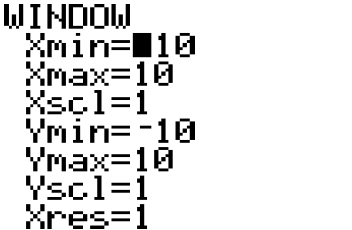
\includegraphics[scale=1.0]{Sections/FunctionsandGraphsImages/Figure21.png}
	%\caption{}
\end{figure}

\textbf{Step 3: Get the graph.} In the upper right corner, you’ll see a key labeled \quotes{GRAPH}. Hit that key now and you should see this:

\begin{figure}[H]
	\centering
	%should be scaled down
	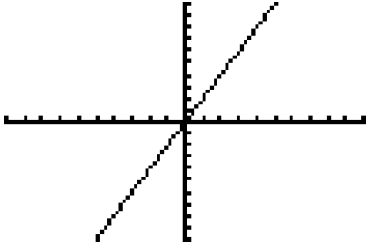
\includegraphics[scale=1.0]{Sections/FunctionsandGraphsImages/Figure22.png}
	%\caption{}
\end{figure}

\index{Calculator:Zoom} As an alternative, when you want a graph in the standard window, you can just hit the \quotes{ZOOM} key in your calculator’s upper row, and select \quotes{6: ZStandard}:

\begin{figure}[H]
	\centering
	%should be scaled down
	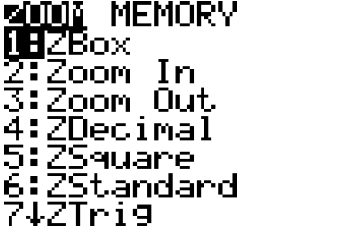
\includegraphics[scale=1.0]{Sections/FunctionsandGraphsImages/Figure23.png}
	%\caption{}
\end{figure}

This will take you directly to the graph in the standard window, essentially combining Step 2 and Step 3.\\

\textbf{It is important to remember that the calculator only shows the portion of the graph that our window instructions tell it to.} It should be apparent that the graph of $f(x)=2x$ continues above and below the graph we generated above. If you wish to see those portions of the graph, you can adjust your window settings and see them. But whether we see them or not, they are there, and while we can’t see them on the calculator’s screen with our actual eyes, we can see them with the mind’s eye. \\

Following these steps, we can now create a graph for just about function defined with a formula.  Our goal is of course not just to admire these graphs’ beauty – we want to use them as a tool, and as we proceed through the course we’ll see more and more how to do this. Before leaving this chapter, though, we’ll mention at least one use for these graphs.\\

Since a function’s graph consists of all its input-output pairs, we can use graphs to find the output for any given input. The calculator allows you to \quotes{walk} along the graph, telling you the coordinates of points you encounter along the way. In the top row of your calculator you will see a key labeled \quotes{TRACE}. If you hit this key, you’ll see a \quotes{blob} placed somewhere on the graph, and the input and output values of its coordinates:

\begin{figure}[H]
	\centering
	%should be scaled down
	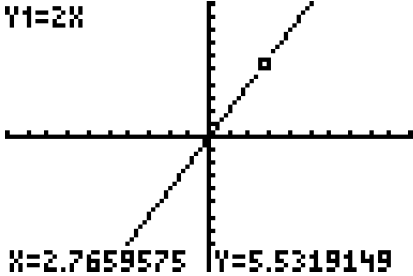
\includegraphics[scale=1.0]{Sections/FunctionsandGraphsImages/Figure24.png}
	%\caption{}
\end{figure}

If you don’t see the coordinate values, hit \quotes{2nd} \quotes{ZOOM} (that is, \quotes{FORMAT}) and make sure your settings are like this:

\begin{figure}[H]
	\centering
	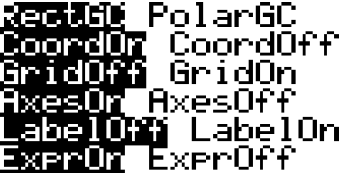
\includegraphics[scale=1.0]{Sections/FunctionsandGraphsImages/Figure25.png}
	%\caption{}
\end{figure}

You can now move around to different points on the graph by using the right and left directional keys in the upper right portion of your calculator.\\

As you do this you’ll notice that not every point on the graph is visited when you trace. That can’t be avoided – there are infinitely many points on the graph, so there’s no way you could visit them all! To visit the point on the graph associated with a given input value, hit \quotes{2nd} \quotes{TRACE} (that is, \quotes{CALC}) in the top row to get this menu:

\begin{figure}[H]
	\centering
	%should be scaled down
	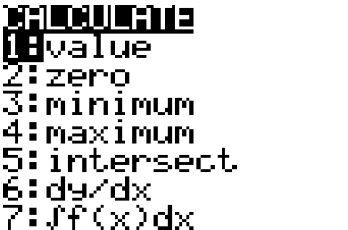
\includegraphics[scale=1.0]{Sections/FunctionsandGraphsImages/Figure26.png}
	%\caption{}
\end{figure}

Select \quotes{1: value} and you’ll be returned to the graph with a screen that looks like this:

\begin{figure}[H]
	\centering
	%should be scaled down
	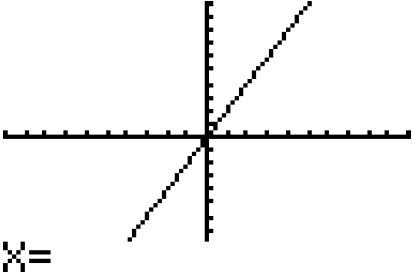
\includegraphics[scale=1.0]{Sections/FunctionsandGraphsImages/Figure27.png}
	%\caption{}
\end{figure}

Now you can enter the input ($x$) value you want to visit. If we want, say, to visit the point that goes with $x=-3$ we get:

\begin{figure}[H]
	\centering
	%should be scaled down
	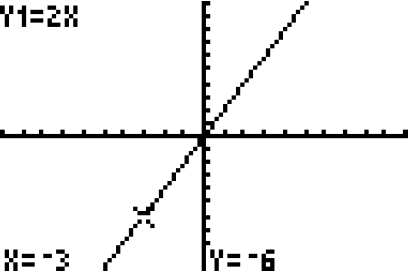
\includegraphics[scale=1.0]{Sections/FunctionsandGraphsImages/Figure28.png}
	%\caption{}
\end{figure}

\exam{\label{FunctionsandGraphsExample8}Obtain a graph for $h(t)=\frac{t^3+3t^2}{12}$ in the standard window, and use this graph to find $h(2)$}

\indenttext{Following the steps outlined above, we first need to enter the function’s formula into the calculator.  Recall that the calculator only understands X as the input value, so we need to rewrite that formula replacing the $t$ with an X:

	\begin{figure}[H]
		\centering
		%should be scaled down
		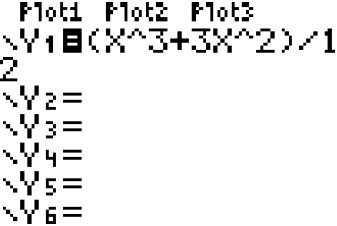
\includegraphics[scale=1.0]{Sections/FunctionsandGraphsImages/Figure29.png}
		%\caption{}
	\end{figure}

	Now, either directly adjusting the window setting to the standard window and hitting \quotes{GRAPH}, or just using \quotes{ZOOM} --> \quotes{6: ZStandard}, we get:

	\begin{figure}[H]
		\centering
		%should be scaled down
		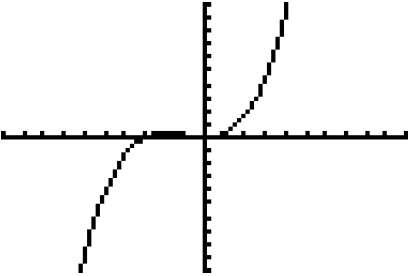
\includegraphics[scale=1.0]{Sections/FunctionsandGraphsImages/Figure30.png}
		%\caption{}
	\end{figure}

	Then using \quotes{2nd} \quotes{TRACE} (that is, \quotes{CALC}) --> \quotes{1: value} and entering \quotes{X=2} we get:

	\begin{figure}[H]
		\centering
		%should be scaled down
		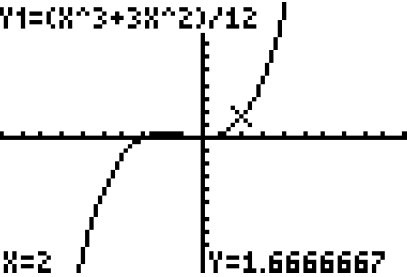
\includegraphics[scale=1.0]{Sections/FunctionsandGraphsImages/Figure31.png}
		%\caption{}
	\end{figure}

	So, we conclude that $h(2)=1.6666667$ which we would either recognize as $h(2)=\frac{5}{3}$ or round t0 something reasonable such as $h(2) = 1.67$.
}

%%%%%%%%%%%%%%%%%%%%%%%%%%%%%%%%%%%%%%%%%%%%%%%%%%%%%%%%%%%%
%
% Functions and Graphs Exercises
%
%%%%%%%%%%%%%%%%%%%%%%%%%%%%%%%%%%%%%%%%%%%%%%%%%%%%%%%%%%%%

\clearpage

\subsection{Exercises}

\subsubsection*{Coordinates}
\ex{Rewrite the function given in the table below as a set of coordinate pairs.
	\begin{center}
		\begin{tabular}{|c|c|c|c|c|c|}
			\hline
			$x$ & 1 & 2 & 4 & 8 & 12 \\
			\hline
			$g(x)$ & 2 & 2 & 7 & 1 & 0\\
			\hline
		\end{tabular}
	\end{center}
} \sol{$\{(1,2), (2,2), (4,7), (8,1), (12,0)\}$}

\bigskip
\ex{Rewrite the function given in the table below as a set of coordinate pairs.
	\begin{center}
		\begin{tabular}{|c|c|c|c|c|c|}
			\hline
			$t$ & 0 & -3 & 6 & 4 & 3 \\
			\hline
			$h(t)$ & 5 & 7 & 6 & 11 & -1\\
			\hline
		\end{tabular}
	\end{center}
}

\bigskip
\ex{Suppose $f(2) = -1$. Express this as a coordinate pair.} \sol{$(2, -1)$}

\bigskip
\ex{Suppose $g(0) = 3$. Express this as a coordinate pair.}

\bigskip
\ex{Rewrite the function given by the following set of coordinate pairs as a table, assume $f(x)$: $\{(1,3), (2,5), (3,-1), (5,-2)\}$.}
\sol{
	$$ \begin{array}{c|c}
		x & f(x) \\
		\hline
		1 & 3 \\
		2 & 5 \\
		3 & -1 \\
		5 & -2 \\
	\end{array} $$}

\bigskip
\ex{Rewrite the function given by the following set of coordinate pairs as a table, assume \( g(t) \): $\{(1,5), (2,-1), (4,6), (7,-3)\}$.}

\bigskip
\ex{The coordinate pair $(5,3)$ gives an input and output for the function $f(x) $.  Does this mean $f(3)=5$ or that $f(5) = 3$?} \sol{$f(5)=3$}

\bigskip
\ex{The coordinate pair $(2, -7)$ gives an input and output for the function $g(t) $. Does this mean $g(2) = -7$ or $g(-7)=2$?}

\bigskip
\ex{Is $\{(0,2), (-1,3), (1, -3), (2,8), (-2, -8)\} $ a function? Why or why not?} \sol{Yes, each input has one and only one corresponding output.}

\bigskip
\ex{Is $\{(0,5), (2,3), (2,5), (4,6), (4,8)\}$ a function? Why or why not?}

\bigskip
\ex{Is $\{(1,1), (2,1), (3,1)\} $ a function?  Why or why not?} \sol{Yes, each input has one and only one corresponding output.}

\bigskip
\ex{Is $\{(1,1), (1,2), (1,3)\} $ a function?  Why or why not?}

\bigskip
\ex{Is $\{(0,0), (0,1), (1,2), (2,3), (3,4)\} $ a function?  Why or why not?}  \sol{No, because the input $0$ has two different outputs ($0$ and $1$).}

\bigskip
\ex{Is $\{(-1,2), (-2,2), (-3,2), (-4,2)\} $ a function?  Why or why not?}

\subsubsection*{Graphs}

\ex{Use your calculator to create a table of values for the function $f(x)=(x+1)(x-1)$ for the inputs $x = -3, -2, -1, 0, 1, 2, 3 $ or create the table yourself by hand.  Then sketch a coordinate plane and plot these points on it.  Use the points you plotted to sketch what the graph of $f(x)$ appears to be.}
\sol{
	$$
	\begin{array}{c|c}
		x & f(x) \\
		\hline
		-3 & 8 \\
		-2 & 3 \\
		-1 & 0 \\
		0 & -1 \\
		1 & 0 \\
		2 & 3 \\
		3 & 8 \\
	\end{array}
	$$
	\begin{figure}[H]
		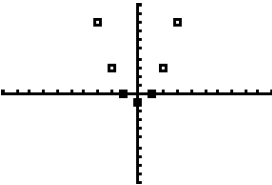
\includegraphics[scale=1.0]{Sections/FunctionsandGraphsImages/Answer15a.png}
	\end{figure}
	\begin{figure}[H]
		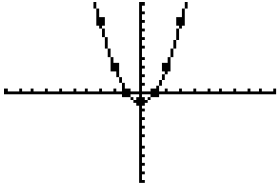
\includegraphics[scale=1.0]{Sections/FunctionsandGraphsImages/Answer15b.png}
\end{figure}}
\bigskip

\ex{Use your calculator to create a table of values for the function $f(x)=x-3(x-1)$ for the inputs $x = -3, -2, -1, 0, 1, 2, 3 $ or create the table yourself by hand.  Then sketch a coordinate plane and plot these points on it.  Use the points you plotted to sketch what the graph of $f(x)$ appears to be.}
\bigskip

\ex{Sketch the location of each of the following points in the Cartesian plan, and state the quadrant in which each is located.
	\begin{enumerate}[label=(\alph*)]
		\item $(2,1)$
		\item $(-1,2)$
		\item $(5,-1)$
		\item $(0,2)$
	\end{enumerate}
}
\sol{
	\begin{enumerate}[label=(\alph*)]
		\item First quadrant
		\begin{figure}[H]
			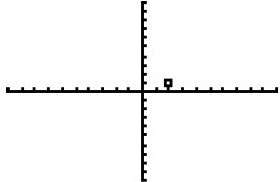
\includegraphics[scale=1.0]{Sections/FunctionsandGraphsImages/Answer17a.png}
		\end{figure}
		\item Second quadrant
		\begin{figure}[H]
			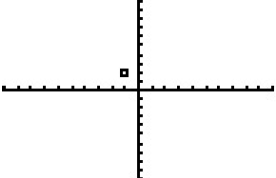
\includegraphics[scale=1.0]{Sections/FunctionsandGraphsImages/Answer17b.png}
		\end{figure}
		\item Fourth quadrant
		\begin{figure}[H]
			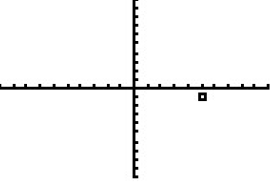
\includegraphics[scale=1.0]{Sections/FunctionsandGraphsImages/Answer17c.png}
		\end{figure}
		\item none, between first and second quadrants
		\begin{figure}[H]
			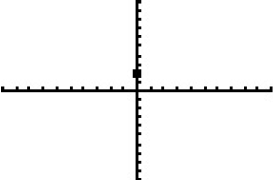
\includegraphics[scale=1.0]{Sections/FunctionsandGraphsImages/Answer17d.png}
		\end{figure}
	\end{enumerate}
}

\bigskip
\ex{Sketch the location of each of the following points in the Cartesian plan, and state the quadrant in which each is located.
	\begin{enumerate}[label=(\alph*)]
		\item $(-3,1)$
		\item $(1,-3)$
		\item $(-1,-3)$
		\item $(-2,0)$
	\end{enumerate}
}

\bigskip
\ex{Sketch a possible graph for each of the functions described. Label your axes, and, if available, include any other relevant information in your graph as well.
	\begin{enumerate}[label=(\alph*)]
		\item the remaining balance on a mortgage as a function of time as the loan is being paid
		\item the monthly sales of hybrid cars as a function of the price per gallon of gasoline
		\item the height of a sunflower as a function of time since the seed was planted 
	\end{enumerate}
}
\sol{Possible graphs, answers will vary
	\begin{enumerate}[label=(\alph*)]
		\item \phantom{a}
		\begin{figure}[H]
			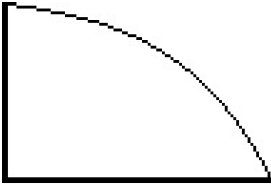
\includegraphics[scale=1.0]{Sections/FunctionsandGraphsImages/Answer19a.png}
		\end{figure}
		\item \phantom{b}
		\begin{figure}[H]
			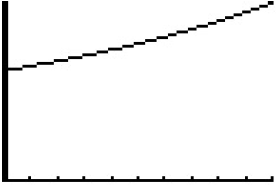
\includegraphics[scale=1.0]{Sections/FunctionsandGraphsImages/Answer19b.png}
		\end{figure}
		\item \phantom{c}
		\begin{figure}[H]
			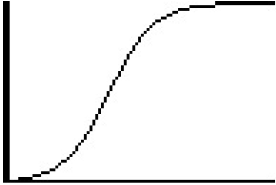
\includegraphics[scale=1.0]{Sections/FunctionsandGraphsImages/Answer19c.png}
		\end{figure}
	\end{enumerate}
}

\bigskip
\ex{Sketch a possible graph for each of the functions described. Label your axes, and, if available, include any other relevant information in your graph as well.
	\begin{enumerate}[label=(\alph*)]
		\item the height of a ball as a function of time since it was thrown upward
		\item the risk of a heart attack as a function of a man’s weight
		\item the amount of oil in a reservoir as a function of time since production from the reservoir began 
	\end{enumerate}
}

\bigskip
\ex{For each of the given scenarios, make a reasonable sketch of what the graph of noise in the college’s basketball area as function of time might look like:
	\begin{enumerate}[label=(\alph*)]
		\item Everyone was excited at the start of the game, since the two teams were bitter rivals in close competition for the league championship. The first half was close, with the two teams pretty well matched and neither team able to get much of a lead. But in the second half, the home team quickly fell behind and never even got close again, finally losing by 18 points.
		\item No one really expected much from this game, since the visiting team was heavily favored, but the home team hung in there and kept the game close through the first half and the first part of the second half. But then the home team had a terrific run and broke away to a 7 point lead. The visitors came back and made it close, taking the lead again just before the buzzer, but the home team put the game away on a last second 3 pointer.
		\item The visiting team already had the league championship locked up, and for the home team this was the last game of a disappointing season. The visitors quickly built up a sizeable lead, and the game never was even competitive.
\end{enumerate} }
\sol{There are many possible answers, but all should show the noise level getting higher when the game is more exciting and lower when the game is less exciting}

\bigskip
\ex{For each of the given scenarios, make a reasonable sketch of what the graph of Zarofire Systems’ stock price might look like as a function of time:
	\begin{enumerate}[label=(\alph*)]
		\item The stock began the year at a price of \$2 per share, and stayed pretty much flat for several months. Then the company reported blow out earnings, and the stock price quickly soared to new highs, after which it continued to rise gradually for the next few months, before leveling off through the end of the year and ending the year at \$10 per share.
		\item The stock began the year at around \$2 per share, and over the first few months of the year slowly and gradually faded downward. About mid–year it started to move upward again for a month or so, approaching but not quite returning to where it started the year, and then leveled off for a few months. Finally, the company unexpectedly filed for bankruptcy, and on that news the stock fell dramatically and ended the year nearly worthless.
		\item The stock began the year at around \$2 per share, and gradually wavered between \$1.75 and \$2.25 for the first half of the year. A bit past midyear, the company received a buyout offer at \$5 per share, and the stock immediately shot up to nearly that price, where it remained until the deal was completed at year’s end.
\end{enumerate} }

\bigskip
\ex{Which of the following could be the graph of a function? Explain your reasoning.
\begin{tabular}{lll}
	a. 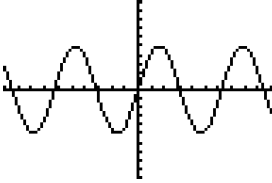
\includegraphics[scale=0.6]{Sections/FunctionsandGraphsImages/Question23a.png}
	&  	
	b. 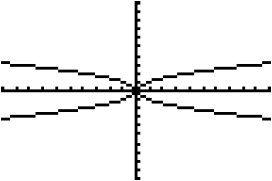
\includegraphics[scale=0.6]{Sections/FunctionsandGraphsImages/Question23b.png}
	&
	c. 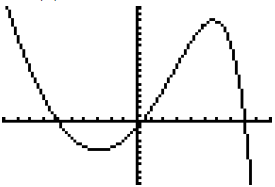
\includegraphics[scale=0.6]{Sections/FunctionsandGraphsImages/Question23c.png}
\end{tabular}
}
\sol{a. is a function  b. is not a function  c. is a function }

\bigskip
\ex{Which of the following could be the graph of a function? Explain your reasoning.
\begin{tabular}{lll}
	a. 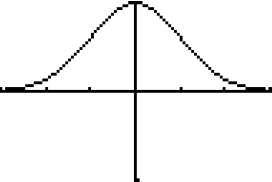
\includegraphics[scale=0.6]{Sections/FunctionsandGraphsImages/Question24a.png}
	&  	
	b. 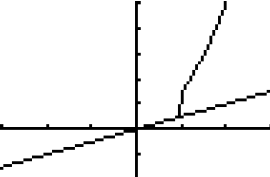
\includegraphics[scale=0.6]{Sections/FunctionsandGraphsImages/Question24b.png}
	&
	c. 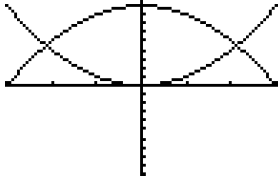
\includegraphics[scale=0.6]{Sections/FunctionsandGraphsImages/Question24c.png}
\end{tabular}
}

\subsubsection*{Graphing Calculator}

\ex{Use your calculator to obtain a graph for $f(x)=5-x$ in the standard window. Use your graph to find $f(2.4)$, $f(-1.3)$, and $f(-7.2)$.}
\sol{$f(2.4)=2.6$, $f(-1.3)=6.3$, and $f(-7.2)=12.2$}

\bigskip
\ex{Use your calculator to obtain a graph for the function $g(x)=7-x/2$ in the standard window. Use your graph to find $g(-3.2)$, $g(1.8)$ and $g(-9.8)$.}

\bigskip
\ex{Use your calculator to create a graph for the function whose graph you sketched in Exercise $15$. Does the calculator’s graph agree with your sketch?}
\sol{The graph should match. (The scale may be different.)}

\bigskip
\ex{Use your calculator to create a graph for the function whose graph you sketched in Exercise $16$. Does the calculator’s graph agree with your sketch?}

\bigskip
\ex{Use your calculator to obtain a graph for the function $h(t)=-16t^2+64t+5$ in the window $0 \leq t \leq 4, 0 \leq h(t) \leq 160$. Use your graph to find $h(1.75)$ and $h(3.8)$.}
\sol{$h(1.75)=68$ and $h(3.8)=17.16$}

\bigskip
\ex{Use your calculator to obtain a graph for the function $j(s)=-4.9s^2+19.6s+2$ in the window $0 \leq s \leq 4, 0 \leq j(s) \leq 75$. Use your graph to find $j(1.75)$ and $j(3.8)$.}

\subsubsection*{Grab Bag}

\ex{If possible, give a value for $q$ that would make the following set of coordinate pairs a function: $\{(0,13), (1,9), (2,14), (q, 9)\}$. If it is not possible to do this, explain.}
\sol{You can use any value except $q=0$ or $q=2$.  If you used $q=1$, then you would have a redundant pair $(1,9)$, but it would still be a function.}

\bigskip
\ex{If possible, give a value for $q$ that would make the following set of coordinate pairs not a function: $\{(0,13), (1,9), (2,14), (q, 9)\}$. If it is not possible to do this, explain.}

\bigskip
\ex{If possible, give a value for $x$ that would make the following set of coordinate pairs a function: $\{(0,1), (1,5), (x, 1)\}$. If it is not possible to do this, explain.}
\sol{You can use any value except $x=1$.}

\bigskip
\ex{If possible, give a value for $x$ that would make the following set of coordinate pairs not a function: $\{(0,1), (1,5), (x, 1)\}$. If it is not possible to do this, explain.}

\bigskip
\ex{Sketch a possible graph for $s(t)$, the speed of your car as a function of time since you got on the thruway.}
\sol{There are several possibilities, but any such graph should show you speeding up when getting on the thruway.  Here is one possibility:
	\begin{figure}[h]
		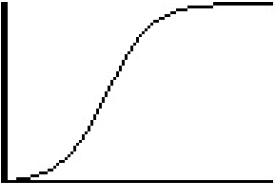
\includegraphics[scale=1.0]{Sections/FunctionsandGraphsImages/Answer35.png}
	\end{figure}
}

\bigskip
\ex{Use your calculator to obtain a graph for $f(x)=10-\frac{x^2}{10}$ in the standard window. Use your graph to find $f(3)$, $f(-5)$, and $f(-8.2)$.}

\bigskip
\ex{Sketch a possible graph for the temperature inside an oven as a function of time since the oven was turned on.}
\sol{There are several possibilities, but any such graph should show the oven starting at room temperature and heating up to the set temperature and pretty much staying at that temperature.  Here is one possible graph:
	\begin{figure}[h]
		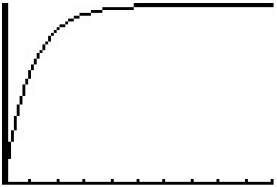
\includegraphics[scale=1.0]{Sections/FunctionsandGraphsImages/Answer37.png}
	\end{figure}
}

\bigskip
\ex{Sketch a possible graph for the temperature inside a hot oven as a function of time since
	the oven was turned off.}

\bigskip
\ex{Use your calculator to obtain a graph for $g(t)=t^3$ in the window $-3 \leq t \leq 3, -50 \leq g(t) \leq 50$}
\sol{The graph
	\begin{figure}[h]
		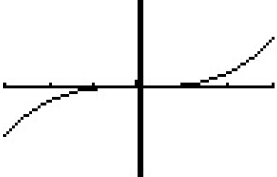
\includegraphics[scale=1.0]{Sections/FunctionsandGraphsImages/Answer39.png}
	\end{figure}
}

\bigskip
\ex{Sketch a possible graph for the volume of water in a backyard pool as a function of the depth of the water in the pool.}

\bigskip
\ex{Use your calculator to obtain a graph for in the standard window for $h(t)=\frac{10-3t}{2}$. Use your graph to find $h(8.2)$, $h(0)$, and $h(-9.6)$.}
\sol{The graph
	\begin{figure}[h]
		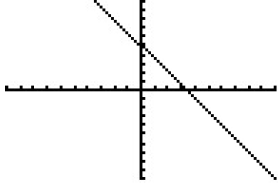
\includegraphics[scale=1.0]{Sections/FunctionsandGraphsImages/Answer41.png}
	\end{figure}
	$h(8.2)=-7.3$, $h(0)=5$, and $h(-9.6)=19.4$}

\bigskip
\ex{Use your calculator to obtain a graph for $p(w)=w-2^w$ in the window $-2 \leq w \leq 4, -20 \leq p(w) \leq 5$.}

\bigskip
\ex{In January, the temperature in Frostbite Falls never went above $0 \deg C$.  Let $f(t)$ be the temperature there as a function of time since the start of the year. If you were to sketch the graph of $f(t)$ for the month of January, in which quadrant would the graph be located?}
\sol{Quadrant IV}

\bigskip
\ex{An agricultural scientist is developing a new fertilizer for corn. She will be conducting a study where different amounts of this fertilizer are applied to several hundred test plots. The expected yield (in bushels) of corn from a test plot is a function of the amount of fertilizer applied (in pounds). The scientist’s expected results are given in the table below:
	\begin{center}
		\begin{tabular}{|c|c|c|c|c|c|}
			\hline
			Fertilizer (pounds) & 0 & 1 & 2 & 3 & 4\\
			\hline
			Expected Yield (bushels) & 5 & 8 & 9 & 8 & 5\\
			\hline
		\end{tabular}
	\end{center}
	Let $x$ be the amount of fertilizer applied, and let $f(x)$ be the expected yield.
	\begin{enumerate}[label=(\alph*)]
		\item Sketch a graph of this function by plotting the points for the data given in the table and making a reasonable guess about the shape of the graph based on these points.
		\item This table gives expected yield as a function of fertilizer applied. Would the actual yield of corn be a function of fertilizer applied? Why or why not?
\end{enumerate} }

\bigskip
\ex{Suppose $p(t)$ is the population of New York City as a function of time since the start of this year. Would the graph of $p(t)$ pass through the origin? Why or why not?}
\sol{No it would not.  The origin is $(0,0)$, so if the graph pass through this point then $p(0)=0$ meaning the population of NYC was 0 at the beginning of the year.}

\bigskip
\ex{Suppose $d(t)$ is the distance I’ve travelled on a road trip as a function of time since I left my house. Would the graph of $d(t)$ pass through the origin? Why or why not? }

\bigskip
\ex{Which of the following shapes could be the graph of a function? Explain your reasoning.
	\begin{enumerate}[label=(\alph*)]
		\item a circle
		\item a horizontal line
		\item a triangle
		\item a semicircle
		\item a vertical line
\end{enumerate} }
\sol{a horizontal line and a semicircle that is either the top half or the bottom half of a circle (any other semicircle would fail to be a function)}

\bigskip
\ex{Which of the following upper-case letters could be the shape of the graph of a function?  Explain your reasoning. 
	\begin{enumerate}[label=(\alph*)]
		\item V
		\item W
		\item E
		\item O
		\item C
\end{enumerate} }

\bigskip
\ex{Suppose $f(5)=-2$. Express this as a coordinate pair.}
\sol{$(5,-2$)}

\bigskip
\ex{The point $(-3,8)$ is on the graph of $g(t)$. Does this mean $g(8)=-3$? Why or why not.}

\bigskip
\ex{The point $(2,7)$ is on the graph of $f(x)$. Does this mean $f(2)=7$? Why or why not.}
\sol{Yes.  The first value is the input and the second value is the output.}

\bigskip
\ex{$f(2)=3$, $f(3)=5$, and $f(5)=2$. Express this as a set of coordinate pairs.}


\clearpage